\documentclass[conference]{IEEEtran}
%\IEEEoverridecommandlockouts
% The preceding line is only needed to identify funding in the first footnote. If that is unneeded, please comment it out.
\usepackage{cite}
\usepackage{amsmath,amssymb,amsfonts}
\usepackage{algorithmic}
\usepackage{graphicx}
\usepackage{textcomp}
\usepackage{xcolor}
\usepackage{subcaption}
\def\BibTeX{{\rm B\kern-.05em{\sc i\kern-.025em b}\kern-.08em
    T\kern-.1667em\lower.7ex\hbox{E}\kern-.125emX}}
\begin{document}

\title{Kalman and Particle filter's robustness to non-linearity}

\author{
    \IEEEauthorblockN{Marius Oechslein}
    \IEEEauthorblockA{
        \textit{Faculty of Computer Science and Business Information Systems} \\
        \textit{University of Applied Sciences Würzburg-Schweinfurt}\\
        Würzburg, Germany \\
        marius.oechslein@study.thws.de
    }
        %\and
}
\maketitle

\begin{abstract}
% TODO: Write this as more of a Zusammenfassung and less of an introduction!

%The Kalman and the Particle filter are often used for estimating the real position of objects based on noisy observations.
% TODO: Also write that it is once again "proven" that the Kalman filter is not able to modle the non-linearities
%In this paper I investigate how non-linearity, like the the impact of a thrown ball with a wall, can be modelled with the Kalman and Particle filter. \\
%While the Kalman filter by definition is only applicable for linear systems, the Particle filter can also be used for non-linear systems.
%Therefore it is interesting to explore how robust the Particle filter is for these kinds of non-linearities. \\
%To investigate the robustness of the Particle filter to non-linearities, the Particle filter is first implemented with low variance and many observations.
%This performance is then compared to an instance with a low amount of observations and an instance with high variance in the observations.
%Since a low amount of observations and high variance is known to have a negative effect on the performance of the particle filter, it will be interesting to see whether the particle model can still model the non-linearity.
\end{abstract}

\begin{IEEEkeywords}
Particle Filter, Kalman Filter, Ball Throw, Non-linearity, Robustness
\end{IEEEkeywords}

\section{Introduction}
The throw of a ball with noisy observations by a 2D camera can be modeled well by the Kalman and Particle filter. 
Both the Kalman and the Particle filter are applicable for this problem due to the uncertainty in the noisy observations.
The Kalman filter by definition is able to model linear systems with high accuracy and the advantage of computationally cheap calculations. 
The Particle filter is also able to model such a problem by recursively estimating the most likely position of the ball over time.

To add non-linearity to this setup, walls are introduced, which change the direction of the ball on impact.
The basic assumptions of the Kalman filter suggest that this can not be modeled well by the Kalman filter.
Therefore it is interesting to examine how well the Kalman filter can still model such a non-linear system. 

The Particle filter on the other hand is popular for use cases with non-linearity \cite{}. % TODO: Cite somewhere that says this.
To investigate the robustness of the Particle filter for non-linear systems, two experiments are conducted.
First the number of observations is decreased and secondly the variance of the observations are increased. 
The point of interest is how the robustness of the Particle filter is affected by this.

% TODO: Irgendwo noch einen Absatz darüber, dass Particle filter das mit den drei Schritten ..., ... und ... rekursiv schafft, die Sachen zu modellen?

% TODO: Überprüfen, mache ich das?
%1. Establishing the research topic \\
%2. Establishing a niche \\
%3. Occupying the niche \\

\section{Physics of a ball throw}
% TODO: Sollte ich hier über die Physics schreiben? Ich glaube, ich könnte schon, wenn ich möchte.
The physics of throwing a ball have to be implemented in the state transition to be able to estimate the position of the ball in the next time step.  
The x-position can be modelled like this:
\begin{equation*}
    \begin{aligned}
    x_{t+1} = x_{t} + v_x * \Delta t,   \\
    x, v_x \in \mathbb{R}
    \end{aligned}
    \tag{1}
\end{equation*}
where the ${v_x}$ is the ball's constant velocity in x-direction and $x_t$ is the x-position of the ball at time step t. \\
The position and velocity in y-direction on the other hand are a bit more complex to calculate since they are affected by gravity.
\begin{equation*}
    \begin{aligned}
    y_{t+1} = y_t + v_y \Delta t - 0.5 g \Delta t^2, \\
    y, v_y \in \mathbb{R}
    \end{aligned}
    \tag{2}
\end{equation*}
with g being the gravity constant at $g = 9.81$. \\
When hitting a wall, the only change in the physical motions is that the velocity in x-direction has to be negated.
So at a after a certain time step where the wall is, the velocity in x-direction has to be updated to this $x^{vel} = -x^{vel}$.
The velocity in y-direction is unchanged with the assumption that there is no fraction when the ball hits the wall and that the wall is exactly vertical. 
The equation for the x-position also remains unchanged.


\section{Kalman and Particle filter}
In this section the Kalman and Particle filter are presented. 
% TODO: equations for the kalman and particles filters
For both the Kalman and Particle filter the hidden state is defined as follows:
\begin{equation*}
\textbf{q} = (x, y, v_x, v_y)   \tag{3}
\end{equation*}
Only the x and y-positions are incorporated in the observations, given by
\begin{equation*}
    \begin{aligned}
    \textbf{o} = (x, y)
    \end{aligned}
\tag{4}
\end{equation*}

Both Kalman and Particle filters implement the following equation for the recursive density estimation:
\begin{equation*}
    p(\textbf{q}_t | \langle \textbf{o} \rangle _t) =
    p(\textbf{o}_t | \textbf{q}_t) \int p(\textbf{q}_t | \textbf{q}_{t-1}) p(\textbf{q}_{t-1} | \langle \textbf{q} \rangle _{t-1}) d \textbf{q}_{t-1}
\tag{5}
\end{equation*}

The Kalman filter does so by the Kalman gain algorithm \cite{b2}.
One important property of the Kalman filter is its linearity assumption.
Due to these assumptions non-linear systems cannot be modelled by the Kalman filter \cite{b2}. % TODO: Stimmt die Citation?
The Particle filter on the other hand can handle non-linearities and can be implemented by the Condensation algorithm \cite{b3}. 


\subsection{Experimental setup}

The first experiment is about a ball throw where the ball hits a wall 50 meter away.
This experiment is conducted to test how well the Kalman and the Particle filter are able to model this non-linearity. 
The outcome of this experiment is expected to be: the Kalman filter not being able to model the non-linearity and the Particle filter being able to model it well.
The point of interest here is specifically how the Kalman filter behaves at the time step where the ball hits the wall and shortly after.  

The second experiment is about the robustness of the Particle filter as the non-linearity of the system increases.
To increase the non-linearity of the system, two further walls are added, where it is interesting to examine whether the Particle filter is able to model the non-linearity as it was for the experiment with only one wall. 
After to seperate changes to the parameters of the systems are made: the number of observations are decreased and the variance of the noise observations are increased.

It was decided to only change the variance and the number of observations, since the main point of interest was how well the Particle filter was able to follow the trajectory of the ball with the ball hitting walls.
Next to the variance and the number of observations, also the noise distribution and assumed starting position could be changed.
These parameters are not changed since the variance the number of observations already give a good intuition of the robustness of the Particle filter and further experiments are therefore not necessary.
All noise was assumed normally distributed and the starting positions were set to the real starting positions of the ball.

% TODO: Different Mathematical Notation ...
%\begin{figure}[h]
%\centerline{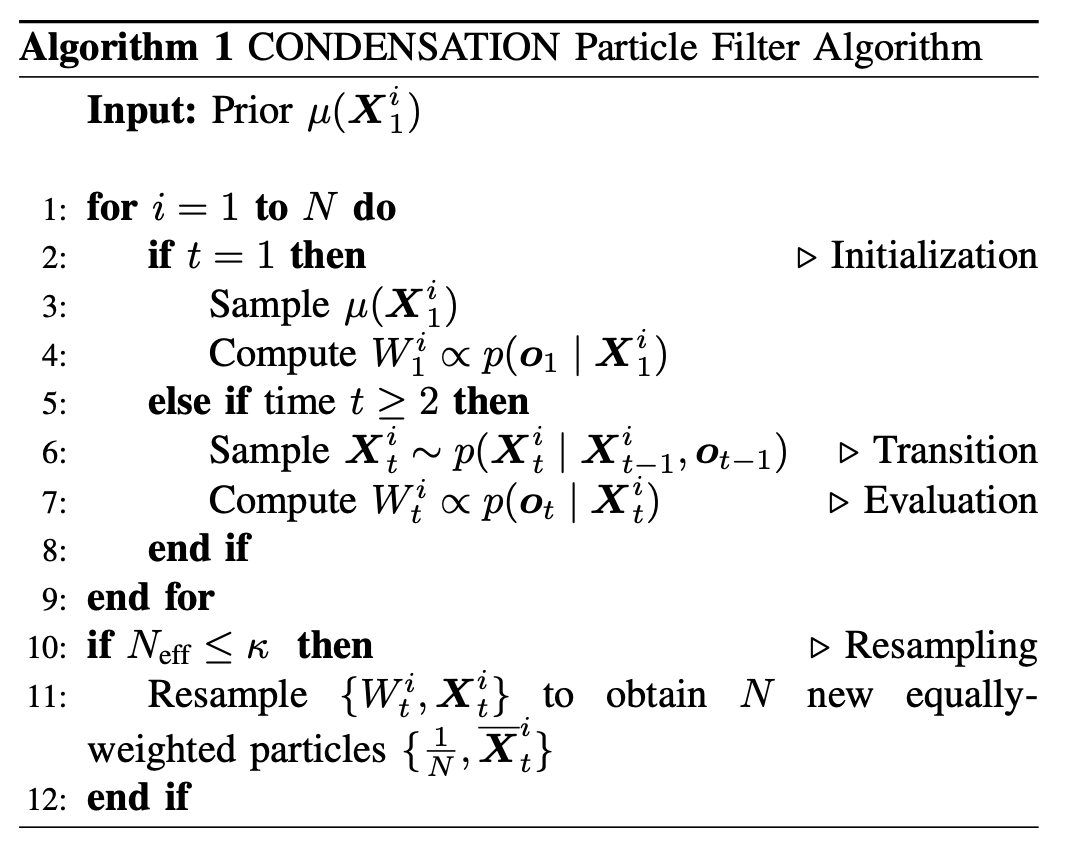
\includegraphics[width=70mm]{figs/condensation-algorithm.png}}
%\caption{Condensation Particle filter algorithm from \cite{b1}.}
%\label{fig:condensation-algorithm}
%\end{figure}

% Structure:
%0. Physics of ball. Also using it for the state transition model later. \\
%1. Simple Math Notations used for Kalman filter \\
%2. Simple Math Notations usef for Particle Filter \\
%3. Somehow introducing the boundaries to Particle Filter math? \\


\section{Results}

% TODO:
% TODO: For all: make sure if it is variance or Standard deviation!

% Kalman filter with time_sim=5, time_step=0.1, variance=1
% Particle filter 1 boundary normal: time=5, time_step=0.1, variance=1
% Particle filter 1 boundary high variance: time=5, time_step=0.1, variance=8 -> 50 observations
% Particle filter 1 boundary few observations: time=5, time_step=0.1, variance=1 -> 12 observations
% Kalman filter 3 boundaries: time_sim=5, time_step=0.1, variance=1
% Particle filter 3 boundaries normal: time=5, time_step=0.025, variance=0.5 -> 200 observations! and lower variance
% Particle filter 3 boundaries higher variance: time=5, time_step=0.025, variance=1 -> way worse for only a little bit more noise
% Particle filter 3 boundaries fewer observations: time=5, time_step=0.1, variance=0.5 -> 50 observations

\subsection{Kalman and Particle Filter modelling non-linearities}

First the results of the Kalman filter estimating the positions of the ball are shown.   
\begin{figure}
	\centering
	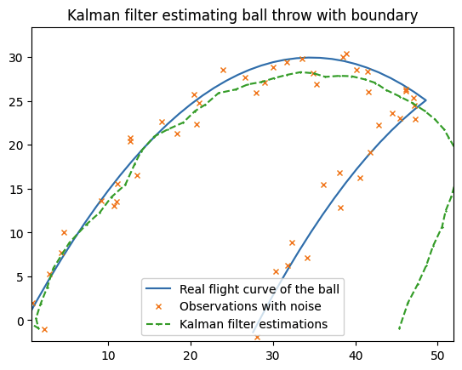
\includegraphics[width=70mm]{figs/kalman-filter.png}
	\caption{Kalman filter modelling non-linearities. From own calculations.}
	\label{fig:kalman-filter}
\end{figure}

In fig. \ref{fig:kalman-filter} the Kalman filter is able to model the trajectory well until the point where the ball hits the wall. 
At this point the estimaitons of the Kalman filter continue on the same trajectory. 
As the errors increase over each time step, the Kalman filter changes its direction slowly, but is never able to come close to the real positions again.

The Particle filter on the other hand is able to model the non-linearity well, as shown in fig. \ref{fig:particle-filter-one-boundary}.
It estimates the positions well before the ball hits the wall and it is able to follow the trajectory of the ball after.

Note that for both experiments the variance of the observation noise and the number of observations are equal to be able to compare the performance of the two filters.  

\begin{table}[htbp]
    \caption{Estimation errors for one boundary. Boundary 50 m away.}
    \begin{center}
    \begin{tabular}{|c|c|c|}
    \cline{1-3}
    & Before hitting the wall & After hitting the wall \\
    \cline{1-3} 
    Kalman filter & \textit{1.2 m} & \textit{17.73 m} \\
    \cline{1-3} 
    Particle filter & \textit{1.87 m} & \textit{3.01 m} \\
    \hline
    \end{tabular}
    \label{tab:comparing-kalman-particle}
    \end{center}
\end{table}

The errors of estimation for the Kalman and Particle filter both increase as the ball hits the wall \ref{tab:comparing-kalman-particle}.
But while the Particle filter is able to estimate with the same error, the Kalman filter's error increases drastically.
Altough the Kalman filter is around 0.5 m more accurate than the Particle filter before the ball hits the wall, this difference is not significant since it could potentially be due to the uncertainty of the system.


\subsection{Robustness of the Particle filter with increasing non-linearity}

In this section I focus on the robustness of the Particle filter as the non-linearity increases, i.e. two more walls are added.
For both of the experiments, the Particle Filter is first tested on reasonable values for the variance of and the number of observations to have a baseline performance.
Later the variance and the number of observations are changed in order to test the robustness of the Particle filter. 

\begin{figure}
	\centering
	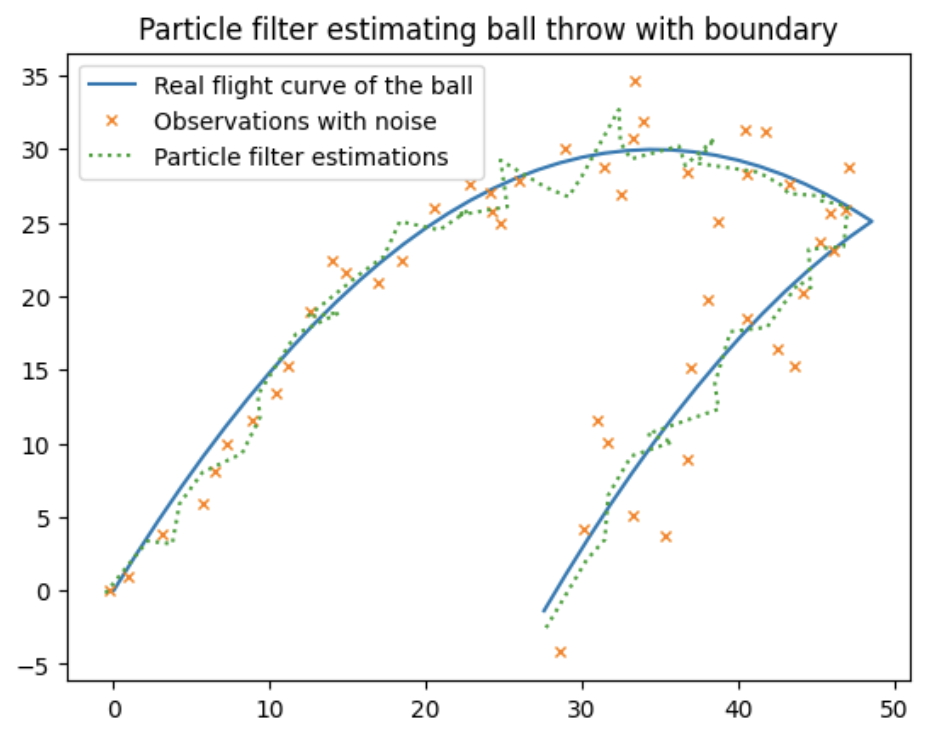
\includegraphics[width=70mm]{figs/particle-filter-one-boundary}
	\caption{Particle filter with one boundary. From own calculations.}
	\label{fig:particle-filter-one-boundary}
\end{figure}
\begin{figure}
	\centering
	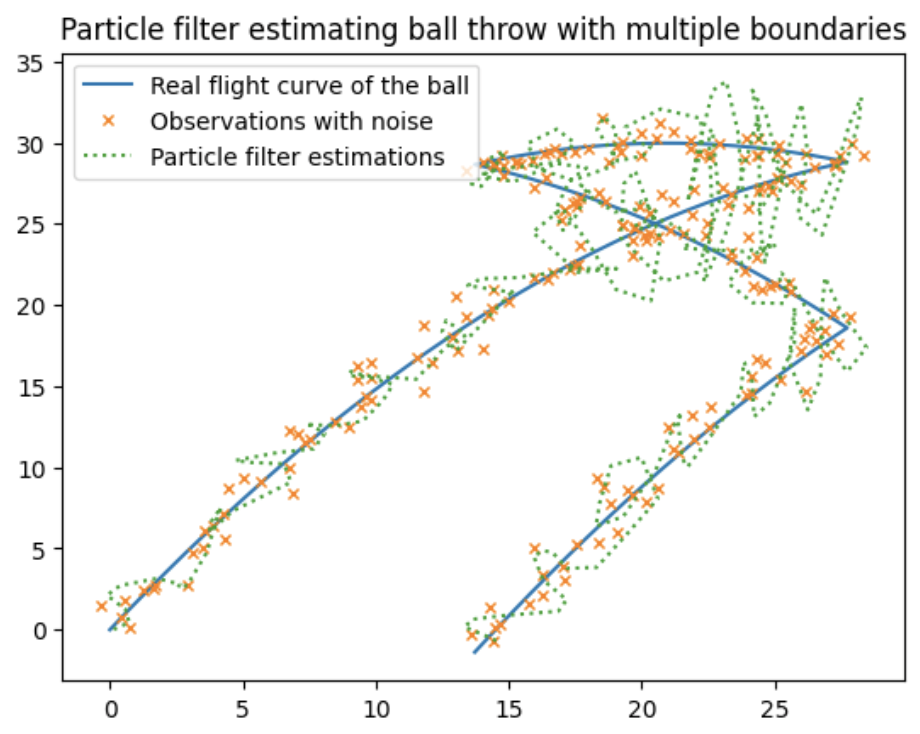
\includegraphics[width=70mm]{figs/particle-filter-multiple-boundaries}
	\caption{Particle filter with multiple boundaries. From own calculations.}
	\label{fig:particle-filter-multiple-boundaries}
\end{figure}

Note that the variance has to be decreased and the number of observations have to be increased substantially when two more walls are added. 
For one wall (fig. \ref{fig:particle-filter-one-boundary}) the variance of the noise is set to 1 and the number of observations are set to 50.
For three walls (fig. \ref{fig:particle-filter-multiple-boundaries}) the variance had to be lowered to 0.025 and the number of observations had to be increased to 200 for the Particle filter to model the balls trajectory reasonably well. \\
This already indicates that the Particle filter struggles to estimate the ball throw as the number of non-linearities increase. 

First the variance of the noise of the observations is increased from 0.025 to 1.
\begin{figure}
	\centering
	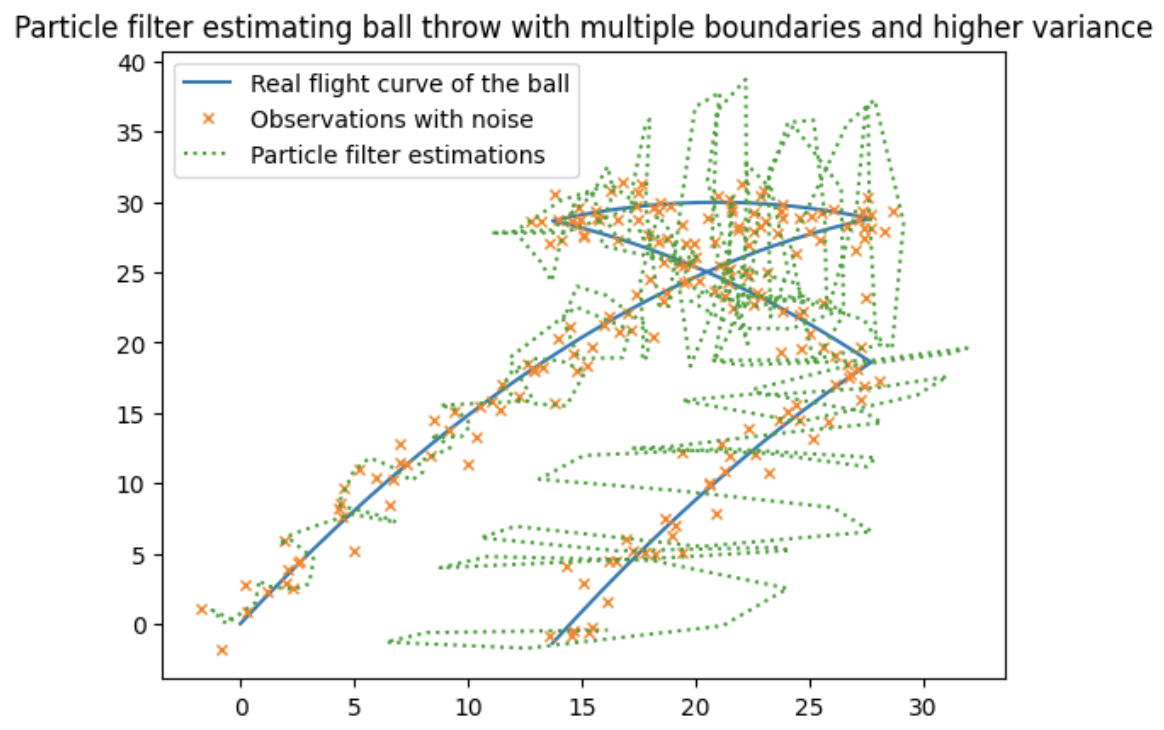
\includegraphics[width=70mm]{figs/particle-filter-multiple-boundaries-higher-variance}
	\caption{Particle filter with multiple boundaries and higher variance. From own calculations.}
	\label{fig:particle-filter-multiple-boundaries-higher-variance}
\end{figure}
Note that this is the same variance that was used for the Particle filter with one boundary in fig. \ref{fig:particle-filter-one-boundary}.
The estimation in fig. \ref{fig:particle-filter-multiple-boundaries-higher-variance} is noticably worse than for the experiment with only one wall, where the same variance for the noise was used.
This indicates that the robustness of the Particle filter decreases as the non-linearity increases.

Secondly the number of observations are decreased from 200 to 50.
Also note here that this is the same number of observations as in fig. \ref{fig:particle-filter-one-boundary} for the Particle filter with one boundary.
\begin{figure}
	\centering
	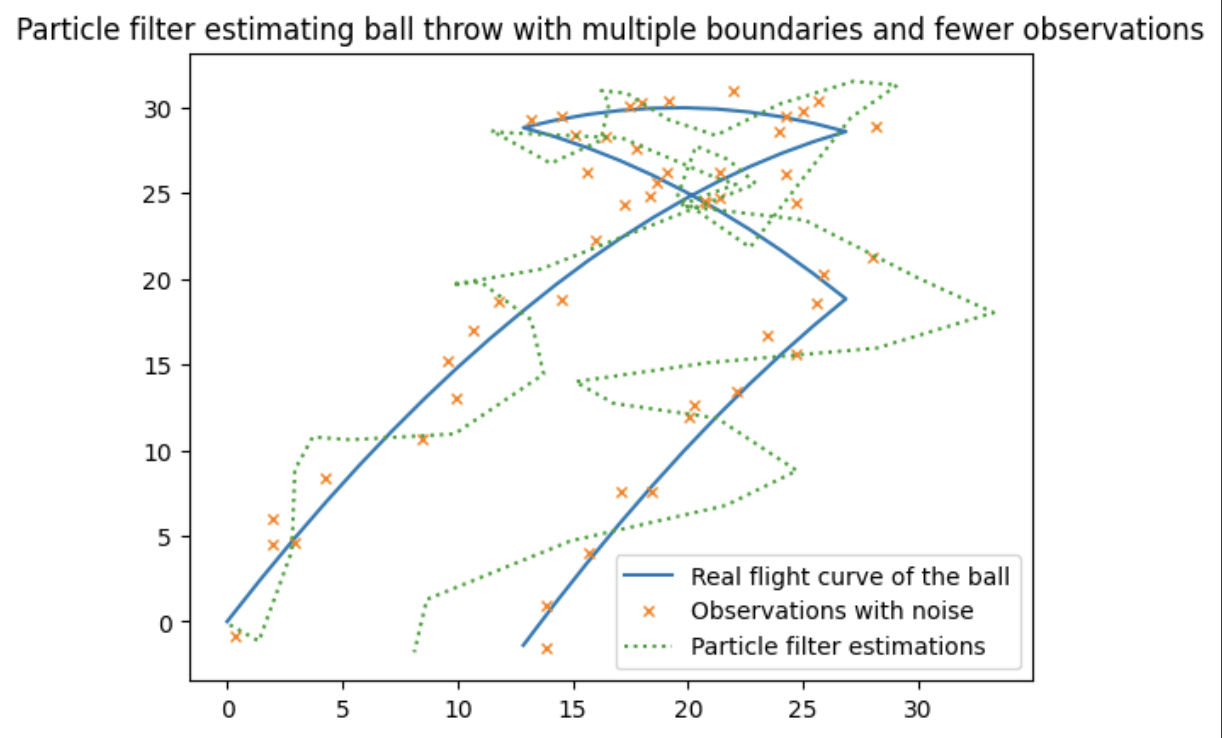
\includegraphics[width=70mm]{figs/particle-filter-multiple-boundaries-fewer-observations}
	\caption{Particle filter with multiple boundaries and fewer observations. From own calculations.}
	\label{fig:particle-filter-multiple-boundaries-fewer-observations}
\end{figure}
Descreasing the number of observations in fig. \ref{fig:particle-fitler-mulitiple-boundaries-fewer-observations} indicate the same resolution as the experiment of increasing the variance: that the robustness of the model decreases as the non-linearity increases.

In conclusion, all of the experiments clearly indicate the the robustness of the Particle filter decreases as the non-linearity increases.


\section{Discussion}\label{sec:discussion}

\subsection{Kalman and Particle Filter modelling non-linearities}

As the basic assumption Kalman filters are linear, the Kalman filter is not able to model such non-linearity.
The same result was observed in the experiments of this study.
Non-linear filters, such as particle filters, unscented Kalman filters, extended Kalman filters, batch filters and exact recursive filters are proposed to handle the problems of the Kalman filter better \cite{b5}.
In this paper I investigated the Particle filter, but the other non-linear filters were not tested. 
For further research it would be interesting to see, whether these other non-linear filters would be able to model the system better.
% TODO: Which of these methods is expected to produce the best results? And why -> cite! Maybe from \cite{b5}: https://ieeexplore.ieee.org/stamp/stamp.jsp?arnumber=1499276&casa_token=hno_g-CsGRoAAAAA:K9RLLHpZgEu-M5qBBobkPgSm1iVZHqhvJ2asLFC4k7XYA2k0f7VckJ-l7IU_nmaZzNKombUiC6z3WA 

\subsection{Robustness of the Particle filter with increasing non-linearity}

The Particle filter was able to model the non-linearity better than the Kalman filter, but as the non-linearity increased, the Particle filter became less robust.  
More observations and less variance in the noise of the observations was required for the Particle filter to still be able to model the system as the non-linearity increased.

There are general known challenges of the Particle filter that could also be the reason for the results of this paper.
The four main challenges of Particles filters concerning the estimation performance are the Degeneracy Problem, Sample Improverishment, Praticle Filter Divergence and selecting the Importance Density \cite{b4}.
In this section I discuss how each of these challenges relates to the observed result that the Particle becomes less robust as the non-linearity increases. 

\subsection{Degeneracy Problem}
The Degeneracy Problem is that after a few iterations most the weight is centered to one particle while all other particles have a weight near zero \cite{b4}.
This problem is solved by an resampling step, where new particles are created based on the weight of the particles from the last iteration.
Since the Condensation Algorithm \cite{b3} is used in the implementation for this paper, this problem is already addressed and thus can not be the reason for the poor results for high non-linearity. 
% TODO: Right? Check the condensation algorithm citation, if this problem is already addressed.

\subsection{Sample Improverishment}
The resampling step used for solving the Degeneracy Problem can become a problem, too.
In the resampling step, particles with high weight are duplicated, which can become a problem, when the state transition does not diversify the new positions of the particles enough \cite{b4}. 
Over time this leads to the problem where all of the particles are condensed into a single position.

This problem is not addressed by the Condensation algorithm used for this implementation and could therefore be a problem in the experiments of this paper. 
For the experiment in fig. \ref{} the number of observations were increased to 200 and the plot indicates that the Particle filter performs much worse as the experiment continues.
This is likely be because of the Sample Improverishment problem, which states that the Particle filter estimates worse over time due to all of the particles collapsing into the same point \cite{b4}. 

Although it is important to note that this problem doesn't necessarily break the Particle filter, for example in fig. \ref{fig:particle-filter-multiple-boundaries} the observations are also increased to 200, but the estimations are close to the real positions.
But this indicates that the Particle filter is not robust for this high non-liniearity, since the estimations get much worse when the variance is increased or the number of observations are decreased unsubstantially the variance is increased or the number of observations are decreased unsubstantially.. 

% TODO: Besser formulieren.
% Ich will sagen, dass es Sinn macht und dass die Plots so aussehen, als könnte das wirklich das Problem sein
% Über die Zeit und besonders nach der ersten boundary im higher-variance plot, werden die estimations um einiges schlechter und die estimations bewegen sich sehr stark pro time step. 
% Das könnte dadurch erklärt werden, dass es über die Zeit immer weniger Particles gibt und irgendwann alle Particles in einer Position sind. 
% Das würde dann dazu führen, dass die Estimations von time step zu time step springen. Und da springt es schnell zu weit, wenn ein Mal eine estimation falsch war.

\subsection{Particle Filter Divergence}

The third problem is the Particle Filter Divergence, where the estimations diverge from the real positions. 
This problem can occur when the filter is poorly tuned, when there are false model assumptions or when there are problems in the measurements \cite{b4}. 

Although the Particle filter struggles to model the systems for high non-linearity, the estimations generally still follow the real position, only with high errors.
This problem can not occur for this application since the throw of the ball is implemented in the state transition and the observations are created artificially, which prevents this problem.  

\subsection{Selecting the Importance Density}
The chosen Importance Density has to fit the system and the Particle filter can only perform well when the Density is appropriately chosen for the problem \cite{b4}. 
This can also not be a porblem, since the underlying gaussian distribution for creating the observations is known and the matching gaussian distribution for the Particle filter was used.


\section{Conclusion}

In this paper experiments were conducted for two points of interest.

The first question was, how exactly the Kalman filter behaves in case of a non-linear system.  
The result for this experiment was that the Kalman filter followed the trajectory of its estimations even though the trajectory of the observations changed direction. 
After the errors of estimation became too big, the Kalman filter changed its direction slowly but never returning to the correct position.

The second question was, how the robustness of the Particle filter is affected when the non-linearity of the system increases.
The result for this experiment was that the Particle filter performed worse when the non-linearity increased. 
This is an interesting conclusion which may be counter intuitive.

For both the Kalman and the Particle filter, there are numerous methods that try to solve the problems of the individual filters. 
While the Particle filter is one of the solutions to the Kalman filter's non-linearity problem, it would be interesting how other methods behave that also try to solve the Kalman filter's problem like the Extended Kalman filter, for example.
For the Particle filter it would also be interesting to see whether other methods that try to solve its problems would be more robust for this use case.


\begin{thebibliography}{00} % TODO: 
	\bibitem{b1} Fetzer, T., Bullmann, M., Ebner, M., Kastner, S., Deinzer, F., \& Grzegorzek, M. Interacting Multiple Model Particle Filter for Indoor Positioning Applications.
	\bibitem{b2} Thrun, S. (2002). Probabilistic robotics. Communications of the ACM, 45(3), 52-57. % TODO: Correct?
	\bibitem{b3} Isard, M., \& Blake, A. (1998). CONDENSATION--conditional density propagation for visual tracking. International journal of computer vision, 29(1), 5.
	\bibitem{b4} Elfring, J., Torta, E., \& van de Molengraft, R. (2021). Particle filters: A hands-on tutorial. Sensors, 21(2), 438.
	\bibitem{b5} Daum, F. (2005). Nonlinear filters: beyond the Kalman filter. IEEE Aerospace and Electronic Systems Magazine, 20(8), 57-69.

\end{thebibliography}

\end{document}
